\documentclass[aps,prd,twocolumn,superscriptaddress,amsmath,amssymb]{revtex4}
\pdfoutput=1
%\usepackage{draftwatermark}
%\SetWatermarkScale{2}
\usepackage{soul}
\usepackage{graphicx}
\usepackage{color}
\usepackage{ulem}
\usepackage{float}
\usepackage{lipsum}

\usepackage{array}
\usepackage{subcaption}
\captionsetup{compatibility=false}
\def\code#1{\texttt{#1}}
\newcolumntype{L}[1]{>{\raggedright\let\newline\\\arraybackslash\hspace{0pt}}m{#1}}
\newcolumntype{C}[1]{>{\centering\let\newline\\\arraybackslash\hspace{0pt}}m{#1}}
\newcolumntype{R}[1]{>{\raggedleft\let\newline\\\arraybackslash\hspace{0pt}}m{#1}}
\newcommand{\lw}{\linewidth}
\usepackage{multirow}

%\usepackage{apacite}
\usepackage{natbib}
%\usepackage[paperwidth=2394pt, paperheight=6840pt]{geometry}
%\SetWatermarkScale{2}
%\SetWatermarkAngle{90}
%\SetWatermarkHorCenter{0.5\paperwidth}
%\SetWatermarkVerCenter{0.5\paperheight}
\begin{document}
%\SetWatermarkLightness{0.5}
\title{Some Title}
\author{S. Carbajal}
\affiliation{Secci\'on F\'isica, Departamento de Ciencias, Pontificia Universidad Cat\'olica del Per\'u, Apartado 1761, Lima, Per\'u}
\author{A.M. Gago}
\affiliation{Secci\'on F\'isica, Departamento de Ciencias, Pontificia Universidad Cat\'olica del Per\'u, Apartado 1761, Lima, Per\'u}

\begin{abstract}
\lipsum[1]
\end{abstract}

\maketitle

\section{TO DO}
\begin{itemize}
\item Mas estadistica para BG (trivial)
\item Falta agregar la parametrizacion de D0 (PYTHIA8). Trivial, pero toma tiempo.
\item Realizar el decay chain para tau leptons. Trivial, pero toma MUCHO tiempo.
\item Falta agregar el decay channel a $\nu K^0$ (trivial)
\item Agregar los 3-body decays de mesones y taus a los scripts config.wls. (trivial)
\end{itemize}
\section{INTRODUCTION}
\lipsum[1]

\section{D meson production}
Heavy neutral leptons (NHLs) with masses above the Kaon mass can be produced in decays of tau leptons, heavy mesons and hadrons. At DUNE energies, however, tau lepton and b-meson productions are heavily supressed, and therefore the only sensible contribution to the heavy neutral lepton fluxe comes from the decays of the charmed mesons $D^\pm$ and $D_s^\pm$. The combined effect of the low $c\bar{c}$ production cross section at DUNE energies combined with the constraints on the values of $|U_\alpha|^2$ heavily supress the expected production of HNL with $m_{\text{HNL}} > m_K$ per POT. In order to mitigate these effects and obtain reasonable statistics, used a Montecarlo simulation to obtain the energies and momenta of the charmed mesons from parametrization formulas. The production cross section of charmed mesons in proton-proton collisions can be parametrized in the Center of Mass frame by the empirical form
\begin{align}
\frac{d^2\sigma}{dx_F dp_T^2} \propto (1-|x_F|)^n e^{-bp_T^2},
\label{eq:paramold}
\end{align}
where $x_F=2p_z\sqrt{s}$, $p_z$ is the longitudinal momentum, $n=6.1\pm0.7$ and $b=1.08\pm0.09$ \cite{alves1996feynman}. However, the values of these parameters were fitted from the E769 experiment, which operated at $E_\text{beam} =250\ \text{GeV}$, at least $100\text{ GeV}$ greater than typical DUNE energies. To study the effects of the energy difference, we simulated fixed-target proton-proton collisions at $E_\text{beam} =120\ \text{GeV}$ in PYTHIA8 \cite{pythia} with the flag \code{"SoftQCD:all"}. As expected, we found that the simulated data is not properly represented by formula (\ref{eq:paramold}). The discrepancy comes from the difference in beam energies between E769 and DUNE, which has an effect on the $c\bar{c}$ production cross section and on the charmed meson production cross section dependence on $x_F$, which is no longer accurately described by $(1-|x_F|)^n$. For this reason, we advice not to use the empirical form (\ref{eq:paramold}) for charmed meson production at DUNE energies.\\
In order to obtain a more reliable parametrization for charmed meson production, we fitted our simulated data to the formula
\begin{align}
\frac{d^2\sigma}{dx_F dp_T^2} \propto \sqrt{\frac{a}{\pi}}e^{-ax_F^2}be^{-bp_T^2},
\label{eq:newparam}
\end{align}
where the $x_F$ dependece is now modeled by a gaussian distribution. The values obtained for the parameters $a$ and $b$ are shown in Table \ref{tab:params} and depend on the flavour of the charmed meson. Fig. \ref{fig:param} shows  our results for $D_s^+$. We note that parametrization (\ref{eq:newparam}), shown in blue, is a reasonably good representation of the data produced by PYTHIA8.

\begin{table}[h]
\begin{center}
\begin{tabular}{|C{0.75cm}|C{2.25cm}|C{2.25cm}|}\hline
\multicolumn{3}{|c|}{FALTA  M\'AS  ESTAD\'ISTICA!} \\ \hline
 & $a\pm\sigma_a$ & $b\pm\sigma_b$ \\ \hline
$D^+$ & $15.192 \pm 0.198$& $0.722 \pm 0.015$ \\
$D^-$ & $13.126 \pm 0.171$& $0.929 \pm 0.021$ \\
$D_s^+$ & $16.634 \pm 0.286$& $0.634 \pm 0.011$ \\
$D_s^-$ & $15.100 \pm 0.352$& $0.800 \pm 0.019$ \\ 
$D^0$ & \textbf{**FALTA} & \textbf{**FALTA }\\ \hline
\end{tabular}
\end{center}
\caption{[FALTA AGREGAR $D^0$] Values of the parameters $a$ and $b$ in parametrization (\ref{eq:newparam}), obtained by fitting to simulated data produced with PYTHIA8.\\
\textbf{** esta bien el sigma o mejor el error con 95\%?}}
\label{tab:params}
\end{table}

\begin{figure}[h]
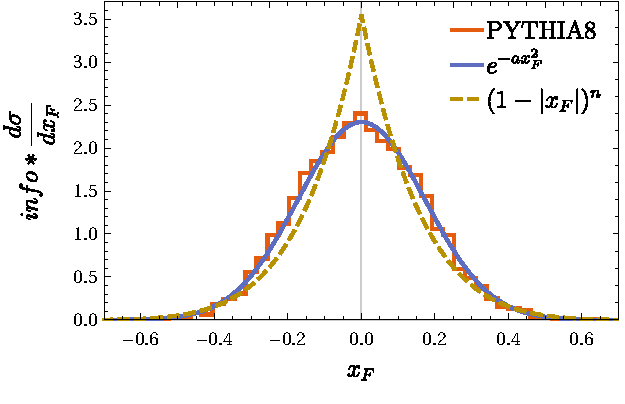
\includegraphics[width=0.9\lw]{plots/plot-fit431xf.pdf}
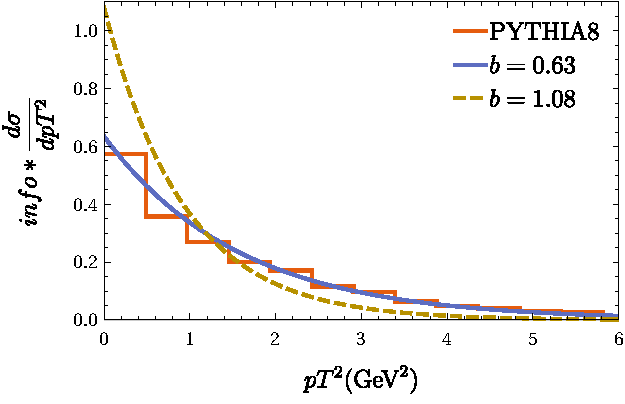
\includegraphics[width=0.9\lw]{plots/plot-fit431pt2.pdf}
\caption{Normalized differential cross sections of $D_s^+$ production in fixed-target proton-proton collisions at $120\text{ GeV}$. Comparison between parametrization formulas (\ref{eq:paramold}) (dashed) and (\ref{eq:newparam}) (solid) is shown.}
\label{fig:param}
\end{figure}

\section{Heavy Neutral Lepton Production}
Heavy neutral Leptons with masses above the Kaon mass can be produced in the decays of charmed mesons and tau leptons via mixing to the standard model neutrinos $\nu_\alpha$. These decays are supressed by the mixing parameters $|U_{\alpha4}|^2$, which are a function of the HNL mass. Several studies have been made to obtain constraints on the mixing parameters \cite{pascoli2019,bondarenko2018, alekhin2016}. In this work, we will use the experimental constraints from \cite{pascoli2019}, which are shown in Figure \ref{fig:mixings}. We will assume that, for each heavy neutral lepton mass, the mixing parameters take the maximum values allowed by these constraints. By doing so, we will calculate the maximum possible variation of the DUNE light neutrino flux due to the presence of heavy neutral leptons with masses above de Kaon mass. The possible production channels also depend on the Dirac or Majorana nature of the HNL. We study both cases separately, since this distinction will affect the number of final light (anti)neutrinos produced by decay of the HNL. We will be particularly interested in the tau neutrino flux since tau neutrinos cannot be produced by decays of lighter mesons.

\begin{figure}[h]
\centering
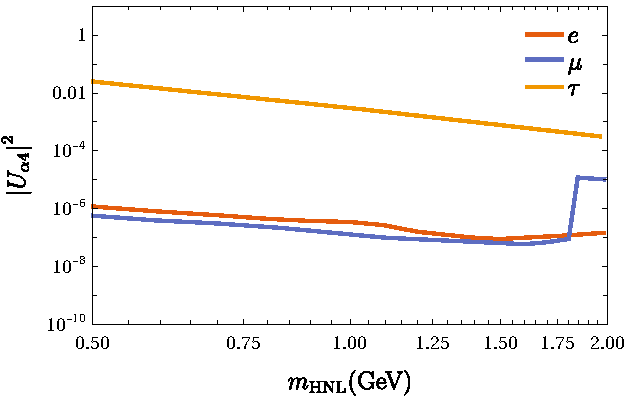
\includegraphics[width=.9\lw]{plots/mixings.pdf}
\caption{Constraints on mixing parameters to heavy neutral leptons for masses above the Kaon mass. The constraints were taken from \cite{pascoli2019} and combine the results of PS191, peak searches, CHARM, NuTeV, DELPHI and T2K.}
\label{fig:mixings}
\end{figure}

\subsection{Production from mesons}

For simplicity, we only simulate the production of heavy neutral leptons via leptonic and semileptnic decays of charmed mesons with braching ratios above $1\%$. These channels are shown in Table \ref{tab:prodchannels}.\\

\begin{table}[h]
\begin{center}
\begin{tabular}{|L{2.cm}L{2.25cm}|L{1.0cm}L{2.0cm}|}\hline
$D^+ \to$ 	& $l_\alpha^+\nu_\alpha$ 										& $\tau^+ \to$ 	&	$\pi^+ \bar{\nu}_\tau$\\
						& $K^0l_\alpha^+ \nu_\alpha$								&  							&	$K^+ \bar{\nu}_\tau$	\\
						& $\bar{K}^*(892)^0l_\alpha^+ \nu_\alpha$	& 							&	$K^*(892)^+ \bar{\nu}_\tau$	\\ 
						& $\bar{K}^*(892)^0l_\alpha^+ \nu_\alpha$ 	& 							&	$\rho(770)^+\bar{\nu}_\tau$	\\ \cline{1-2}
$D^0 \to$ 	& $K^-l_\alpha^+\nu_\alpha$ 								& 							&	$\bar{\nu}_\tau l_\alpha^-\bar{\nu}_\alpha$	\\
\textbf{**FALTA}						& $K^*(892)^-l_\alpha^+\nu_\alpha$ 		& 							&	$\pi^+ \pi^0 \bar{\nu}_\tau$	\\ \cline{1-2}
$D_s^+ \to$ & $l_\alpha^+\nu_\alpha$ 									& 							&		\\
						& $\eta l_\alpha^+ \nu_\alpha$ 							& 							&		\\ 
						& $\eta' l_\alpha^+ \nu_\alpha$ 						& 							&\\
						& $\phi l_\alpha^+ \nu_\alpha$  						& 							& \\ \hline										
\end{tabular}
\end{center}
\caption{Channels considered for the production of heavy neutral leptons. Charged conjugate channels are also considered when necessary.\\
\textbf{**anadir data de maxima mHNL?}\\
\textbf{**cambiar el estilo de la tabla?}}
\label{tab:prodchannels}
\end{table}

Having selected the most relevant HNL production channels, we calculated the width for each of them using the formulas from Ref. \cite{bondarenko2018}. For instance, the partial width for the production of a Dirac HNL via the leptonic decay $P\to l_\alpha N$ of a charmed pseudoscalar meson $P$ with quark composition $\left|P\right>=\left|\bar{U}D\right>$ is given by
\begin{align}
\begin{split}
\Gamma(P\to l_\alpha N)=&\frac{G_F^2f_P^2m_P^2}{8\pi}|V_{UD}|^2|U_{\alpha4}|^2\\
&\times \left[y_N^2+y_l^2-(y_N^2-y_l^2)^2 \right]\sqrt{\lambda(1,y_N^2,y_l^2)},
\end{split}
\label{eq:widthleptonic}
\end{align}
where $f_P$ is the decay constant of the parent meson, $m_P$ its mass, $V_{UD}$ the relevant CKM matrix, $U_{\alpha4}$ the mixing parameter, $y_i=\frac{m_i}{m_P}$ and $\lambda$ is the K\"all\'en function \cite{kallen1965elementary} defined by
\begin{align}
\lambda(a,b,c)=a^2+b^2+c^2-2ab-2ac-2bc.
\end{align}
Fig. \ref{fig:br431} shows the maximum branching ratios for $D_s^+\to l_\alpha N$ allowed by the experimental constraints on the mixing parameters. The bump at $m_{HNL}\sim 1.8GeV$ comes from a sudden decrease in the constraints of $|U_{\mu4}|^2$.\\

\begin{figure}[h]
\centering
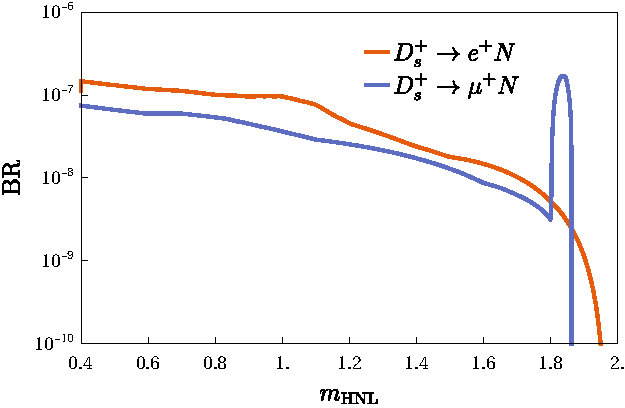
\includegraphics[width=.9\lw]{plots/br431.pdf}
\caption{Maximum branching ratios for $D_s^+\to l_\alpha^+ N$ allowed by the current experimental constraints on the mixing parameters.}
\label{fig:br431}
\end{figure}

The equations for the partial widths of semileptonic decays of pseudoscalar mesons are rather cumbersome, so we refer the reader to Ref. \cite{bondarenko2018}. The production of HNLs via semileptonic decays involve hadronic currents that cannot be calculated from first principles due to the non-perturbative nature of QCD at low energies. Therefore, the dynamics of these decays are modeled by form factors that represent the momentum distribution of the quarks inside the mesons and parametrize the momentum transfer between the hadronic current and the lepton pair \cite{richman1995leptonic}. For most of the semileptonic decays in Table \ref{tab:prodchannels}, we used the form factors presented in \cite{bondarenko2018}. The only exception was the decay $D_s^+\to\phi l_\alpha^+\nu_\alpha$, where we used the parametrizations of the form factors from \cite{aliev2004form}. In order to confirm the validity of our results, we set $m_{\text{HNL}}=0$ and $|U_{\alpha4}|^2=1$ and confirmed that all the branching ratios agreed with the experimental values for decays of charmed mesons into light neutrinos \cite{pdg2018}. We assume that the heavy meson decays are sufficiently prompt that the effects of the pressence of magnetic horns at DUNE can be neglected.

\subsection{Production from tau lepton}

Heavy neutral leptons with masses above the Kaon mass can also be produced via tau decays. However, at DUNE energies tau production directly from $pp$ collisions is heavily suppresed. Therefore, we consider only tau leptons produced in the decays of charmed mesons. Table \ref{tab:prodchannels} shows the decay channels considered for the tau lepton. The formulas for the decay widths that involve mesons in the final state were taken from \cite{bondarenko2018} and formulas for pure leptonic decays from \cite{shaposhnikov2007}. Again, we assume that the production and decay of the tau leptons are suffitiently prompt that the effects of magnetic horns can be neglected. The decay channel $\tau^+\to \pi^+\pi^0\bar{\nu}_\tau$ was considered only at the phase space level.

\section{HEAVY NEUTRAL LEPTON DECAY}
\textbf{**Agregar mas referencias en la distincion entre Dirac/Majorana}\\

After their production, the heavy neutral leptons propagate a small distance and then decay on flight via mixing with light neutrinos. Table \ref{tab:hnldecays} shows all the decay channels for the HNLs considered in this work. We included all the kinematicaly allowed decays to final states involving pseudoscalar and vector mesons as well as pure leptonic decays \cite{pascoli2019}. We used the formulas for the partial decay widths of heavy neutral leptons presented in \cite{bondarenko2018} to find the branching ratios for each decay channel. 
\begin{table}[h]
\begin{center}
\begin{tabular}{|C{1.5cm}|C{1.5cm}|C{1.5cm}|C{1.5cm}|}\hline
$l_\alpha^-\nu_\beta l_\beta^+$ 
	&  $\nu_\alpha \nu_\alpha \bar{\nu}_\alpha$ 
	& $\nu_\alpha\pi^0$ 
	& $l_\alpha^-\rho^{+}$\\
$\nu_\alpha l^+_\beta l^-_\beta$  
	& $l_\alpha^-\pi^+$ 
	& $\nu_\alpha\eta$ 
	& $\nu_\alpha\rho^0$\\
$\nu_\alpha l^+_\alpha l^-_\alpha$ 
	& $l_\alpha^-K^+$ 
	& $\nu_\alpha\eta'$ 
	& $\nu_\alpha\omega$\\
$\nu_\alpha \nu_\beta \bar{\nu}_\beta$ 
	& $l_\alpha^-D^+$ 
	& $l_\alpha^-K^{*+}$ 
	& $\nu_\alpha\phi$\\ \hline
\end{tabular}
\end{center}
\caption{Heavy neutral lepton decay channels considered in this work. \\ \textbf{**falta agregar el canal} $\nu_\alpha K^0$}
\label{tab:hnldecays}
\end{table}

The branching ratios involving a final lepton $l_\alpha$ or light neutrino $\nu_\alpha$ depend on the values of the mixing parameters $U_{\alpha4}$. Again, we assume that the mixing parameters take their maximum experimentally allowed values and calculate the branching ratios accordingly. Figs. \ref{fig:brCCNC} shows the branching ratios for charged current and neutral current mediated decays for $|U_\alpha|^2=1$. Our results mostly agree with \cite{pascoli2019}, although small differences between some branching rations were found. The source of the discrepancy is unknown. 

\begin{figure}[h]
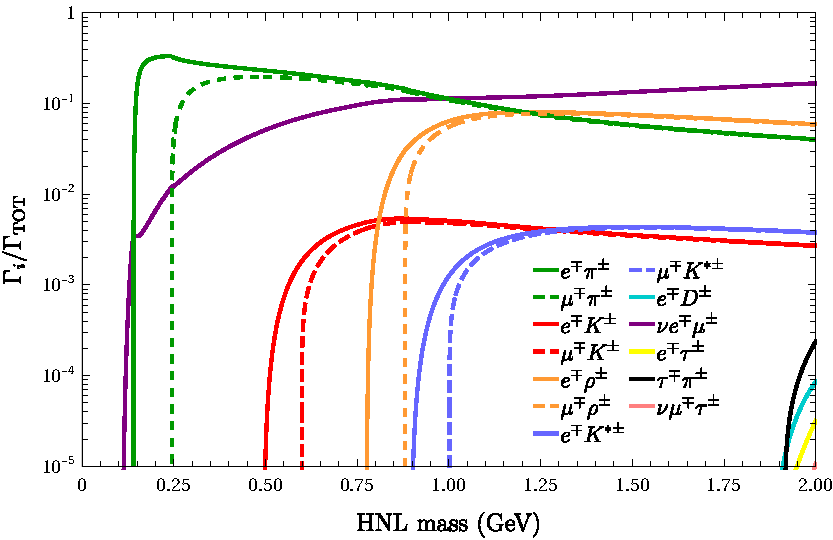
\includegraphics[width=\lw]{plots/plotCC.pdf}
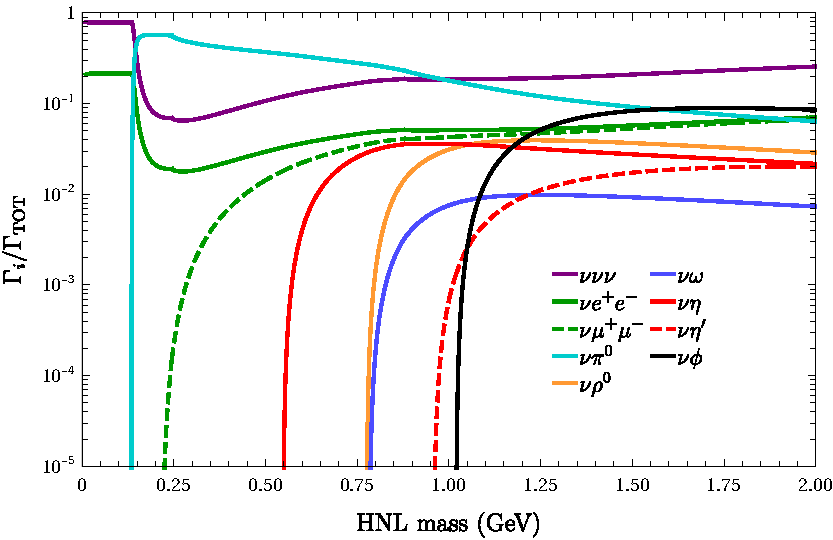
\includegraphics[width=\lw]{plots/plotNC.pdf}
\caption{Branching ratios of charged current (top) and neutral current (bottom) mediated decays of HNLs for $|U_\alpha|^2=1$. The branching ratios do not depend on the Dirac or Majorana nature of the HNL.\\
\textbf{**esta bien este plot o seria mejor hacerlo con los constraints para los mixing?}}
\label{fig:brCCNC}
\end{figure}

It is important to note that the branching ratios presented in Fig. \ref{fig:brCCNC} do not depend on the Dirac or Majorana nature of the HNL. This is because we are plotting the combination of each channel with its respective charged-conjugate process, effectively cancelling out any factors of two that might appear. However, these factors of two are important to determine the partial widths of each channel \cite{pascoli2019}. For instance, a Dirac HNL can decay to charged pions only via $N\to e^-\pi^+$, but a Majorana neutrino can also decay through $N\to e^+\pi^-$. This  evidently has an effect on the rates of $\pi^+/\pi^-$ production from HNL decays, but does not affect the partial decay widths. This means that CC mediated channels have the same partial widths for Dirac and Majorana neutrinos:
\begin{align}
\begin{split}
\Gamma(N_M\to l^- X^+)=\Gamma(N_D\to l^- X^+),\\
\Gamma(N_M\to l^+ X^-) = \Gamma(\bar{N}_D\to l^+ X^-).
\end{split}
\label{eq:relwidthsCC}
\end{align}
On the other hand, NC mediated channels do distinguish between Dirac and Majorana HNLs. This is because the contractions of the NC operator add an additional contribution to the differential decay width of the Majorana HNL,
\begin{align}
d\Gamma(N_M\to \nu X) = d\Gamma(N_D\to \nu X) + d\Gamma(\bar{N}_D\to \bar{\nu} X).
\end{align}
Therefore, a factor of 2 appears when comparing the partial widths of NC mediated decays,
\begin{align}
\Gamma(N_M\to \nu X) = 2\Gamma(N_D\to \nu X).
\label{eq:relwidthsNC}
\end{align}
Equations (\ref{eq:relwidthsCC}) and (\ref{eq:relwidthsNC}) imply that the total widths of Majorana and Dirac HNLs are related by
\begin{align}
\Gamma_\text{T}(N_M)=2\Gamma_T(N_D),
\end{align}
which translates into a difference between their lifetimes,
\begin{align}
\tau(N_M)=\frac{1}{2}\tau(N_D).
\end{align}

\section{Implementation of Production and decay of HNL in PYTHIA8}
With the information of the branching ratios for all the production and decay channels of HNLs, we designed a script that takes as input the mass of the HNL and generates configuration files for PYTHIA8. These files contain all the information that PYTHIA8 needs to simulate the propagation and decays of the charmed mesons, the propagation and decays of the HNLs and the decays of all final unstable particles. We preserved the decay modes of the charmed mesons and the tau lepton by setting the \code{meMode} parameters to the default values used by PYTHIA8 for decays into active neutrinos. The decay modes of the HNLs were set to pure phase space, which is equivalent to averaging over helicity states. We leave the treatise of helicity depence for a future work.\\

The initial energies and momenta of the charmed mesons were obtained with a montecarlo simulation according to the differential cross section (\ref{eq:paramold}) and the parameters of Table \ref{tab:params}. Given a dataset of charmed mesons' energy and momenta and the relevant configuration files, we let PYTHIA8 simulate all the decay chain, up to the production of active neutrinos. Finally, the data of all active neutrinos was saved for further analysis. 

\section{Detection at dunend}

[info general acerca de DUNE, DUNEND, DUNEMPD y DUNE PRISM]\\

For HNL masses in the range , we determined the active neutrino flux on the DUNEND and the MPD detector at different off-axis positions. The

\section{RESULTADOS PRELIMINARES}

\subsection{background}
\noindent
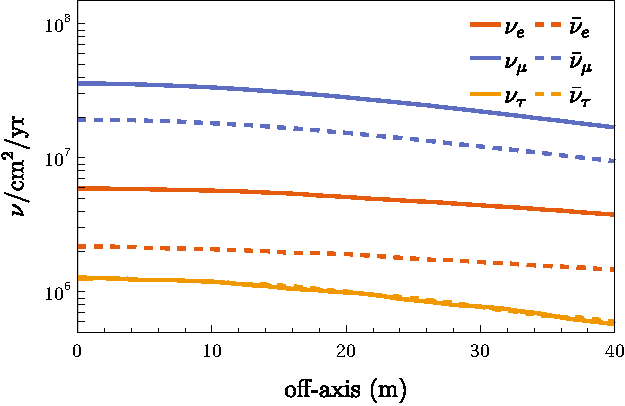
\includegraphics[width=\lw]{plots/meeting/meta.pdf}
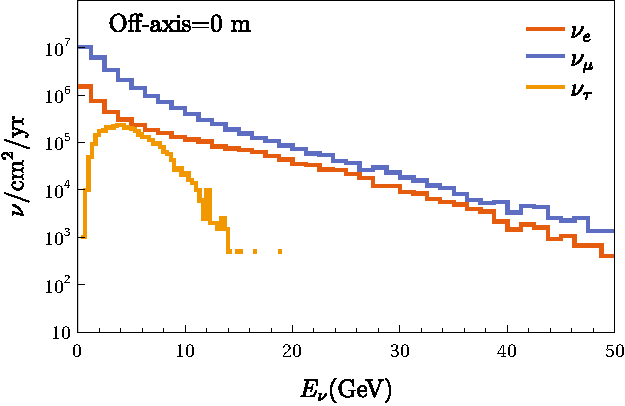
\includegraphics[width=\lw]{plots/meeting/energy-0.pdf}
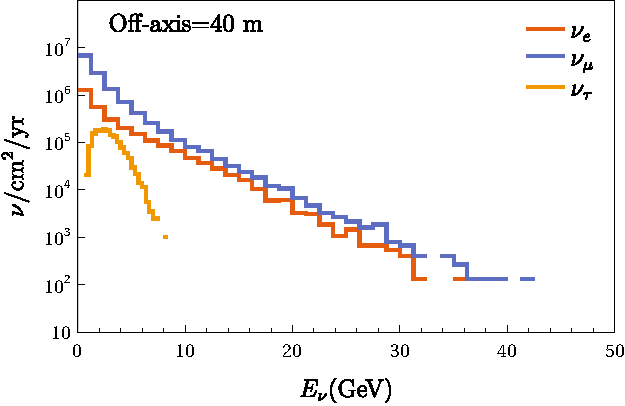
\includegraphics[width=\lw]{plots/meeting/energy-40.pdf}
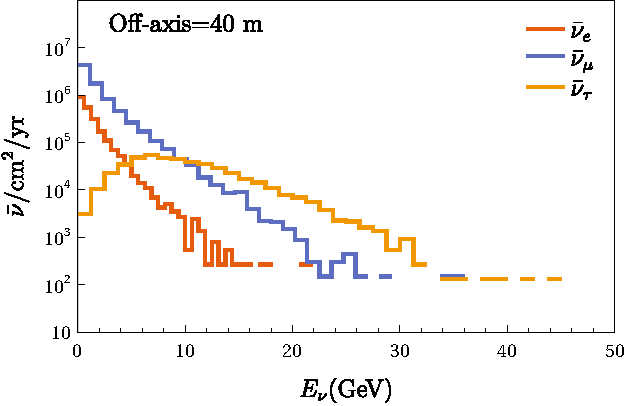
\includegraphics[width=\lw]{plots/meeting/energybar-40.pdf}
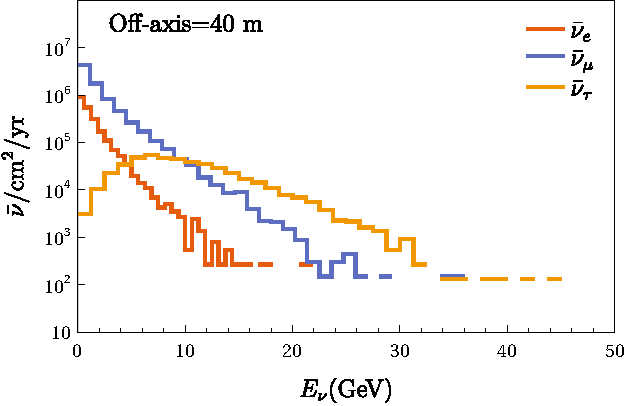
\includegraphics[width=\lw]{plots/meeting/energybar-40.pdf}
\newpage

\subsection{with HNL}
\noindent
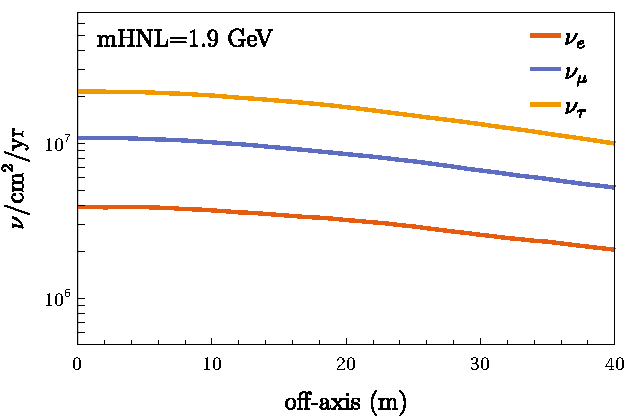
\includegraphics[width=\lw]{plots/meeting/431-meta-19.pdf}
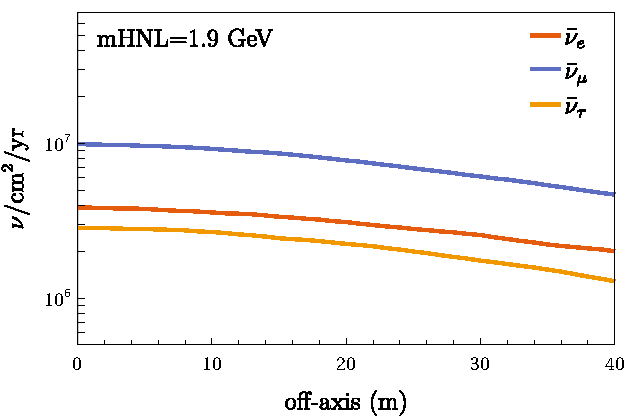
\includegraphics[width=\lw]{plots/meeting/431-metabar-19.pdf}
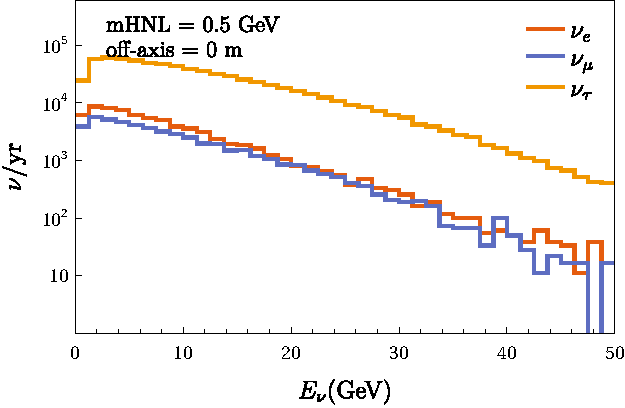
\includegraphics[width=\lw]{plots/meeting/e-05-0.pdf}
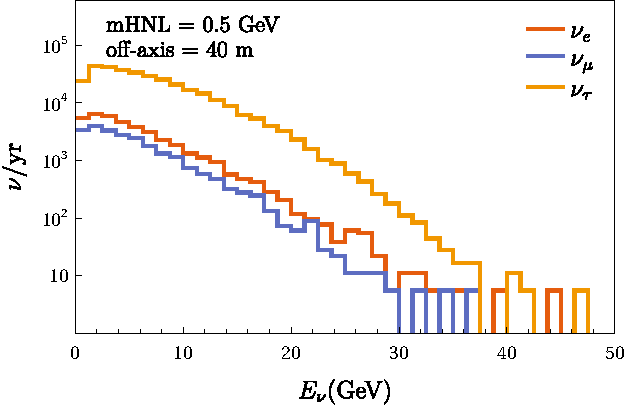
\includegraphics[width=\lw]{plots/meeting/e-05-40.pdf}
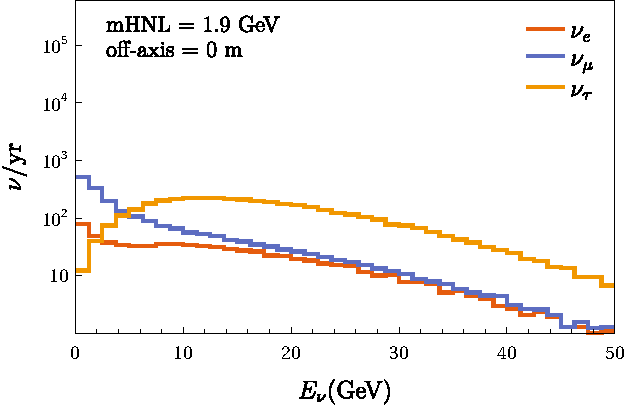
\includegraphics[width=\lw]{plots/meeting/e-19-0.pdf}



















\bibliography{biblio}

\end{document}
